% begin module diff-eq-natural-growth-solution
\begin{frame}
\begin{columns}[c]
\column{.4\textwidth}
\[
\frac{\diff P}{\diff t} = k P
\]
\column{.6\textwidth}
\ \only<handout:0| -9>{%

\includegraphics[height=4cm]{diff-eq-models/pictures/10-01-natgrowtha.pdf}%
}%
\only<handout:0| 10>{%
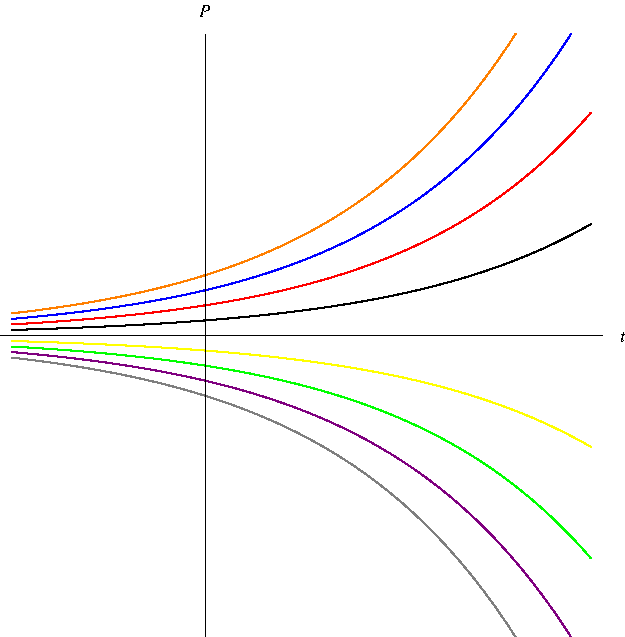
\includegraphics[height=4cm]{diff-eq-models/pictures/10-01-natgrowthb.pdf}%
}%
\only<11->{%
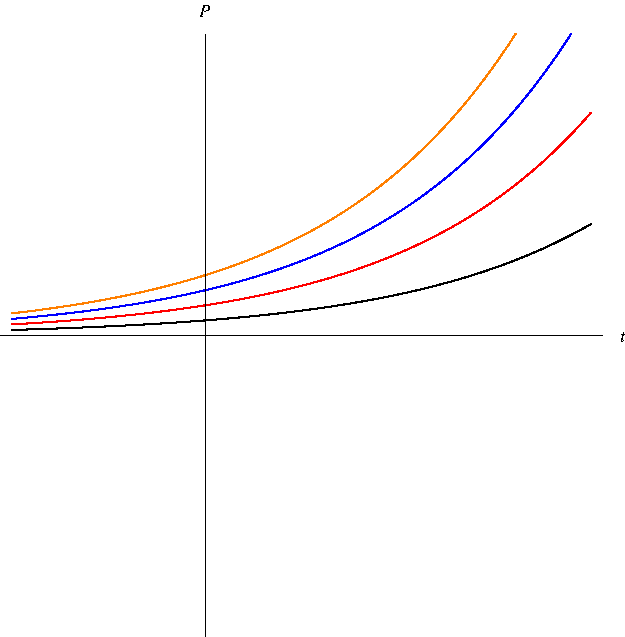
\includegraphics[height=4cm]{diff-eq-models/pictures/10-01-natgrowthc.pdf}%
}%
\end{columns}
\begin{itemize}
\item  This is a differential equation.
\item<2->  Exponential functions satisfy this condition.
\item<3->  Let $\alert<handout:0| 8>{P(t) = Ce^{kt}}$ ($C$ is a constant).  Then
\abovedisplayskip=0pt
\belowdisplayskip=0pt
\[
\uncover<4->{%
\frac{\diff P}{\diff t} = %
}%
\uncover<5->{%
\frac{\diff}{\diff t} (Ce^{kt}) = %
}%
\uncover<6->{%
 Cke^{kt} = %
}%
\uncover<7->{%
 k\alert<handout:0| 8>{Ce^{kt}} = %
}%
\uncover<8->{%
 k\alert<handout:0| 8>{P(t)} %
}%
\]
\item<9->  Therefore any function of the form $P(t) = Ce^{kt}$ satisfies the equation.  We will see later that there is no other solution.
\item<10->  Letting $C$ vary over the real numbers gives a family of solutions.
\item<11->  Populations have positive values, so we only care about $C > 0$.
\end{itemize}
\end{frame}
% end module diff-eq-natural-growth-solution
